\documentclass{standalone}
\usepackage{tikz}

\begin{document}
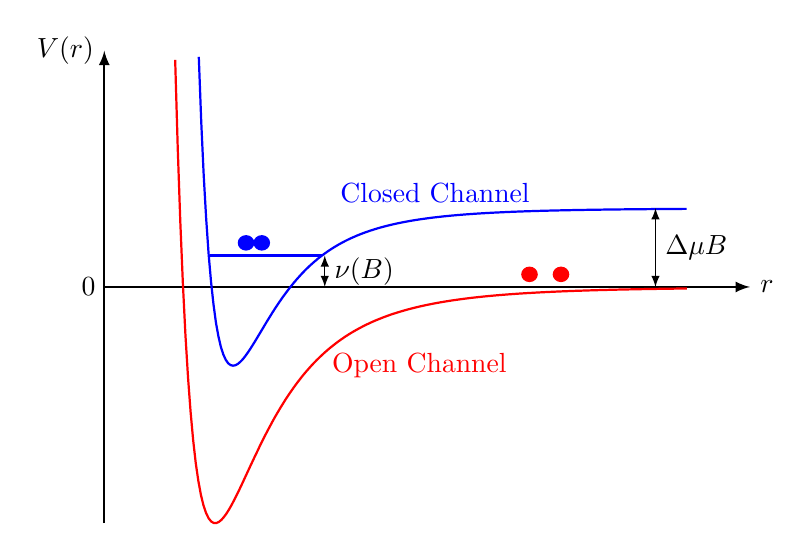
\begin{tikzpicture}[scale=2]

% Diagram axis
\draw[-latex, thick] (0.5,0) -- (4.6,0) node[right] {$r$};
\draw[-latex, thick] (0.5,-1.5) -- (0.5,1.5) node[left] {$V(r)$};
\draw[thick] (0.4,0) node[align=center] {0};

% Lennard-Jones potential (blue)
\draw[domain=1.1:4.2, samples=200, variable=\x, blue, thick] plot (\x, {4*((1/(0.7*\x+0.2))^12 - (1/(0.7*\x+0.2))^6)+0.5});
% Closed channel (blue)
\draw[blue, thick] (2.6,0.6) node[align=center] {Closed Channel};

\fill[blue, thick] (1.4,0.28) ellipse (1.5pt and 1.4pt);
\fill[blue, thick] (1.5,0.28) ellipse (1.5pt and 1.4pt);
\draw[blue, thick] (1.17,0.2) -- (1.88,0.2);

% Lennard-Jones potential (red)
\draw[domain=0.95:4.2, samples=200, variable=\x, red, thick] plot (\x, {6*((1/(0.6*\x+0.4))^12 - (1/(0.6*\x+0.4))^6)});
% Open channel (red)
\draw[red, thick] (2.5,-0.5) node[align=center] {Open Channel};

\fill[red, thick] (3.2,0.08) ellipse (1.5pt and 1.4pt);
\fill[red, thick] (3.4,0.08) ellipse (1.5pt and 1.4pt);

% Resonant coupling arrow
\draw[latex-latex] (4,0) -- (4,0.5) node[midway, right] {$\Delta\mu  B$};
\draw[latex-latex] (1.9,0) -- (1.9,0.2) node[midway, right] {$\nu(B)$};


\end{tikzpicture}
\end{document}